\documentclass[12pt,a4paper]{report}

%===============================================================================
% PACKAGES
%===============================================================================
\usepackage[margin=1in]{geometry}
\usepackage{tikz}
\usepackage{booktabs}
\usepackage{tabularx}
\usepackage{colortbl}
\usepackage{multirow}
\usepackage{hyperref}
\usepackage{xcolor}
\usepackage{titlesec}
\usepackage{enumitem}
\usepackage{fancyhdr}
\usepackage{float}
\usepackage{tcolorbox}
\usepackage{amsmath}
\usepackage{amssymb}
\usepackage{mathtools}
\usepackage{array}
\usepackage{graphicx}
\usepackage{pgfplots}
\pgfplotsset{compat=1.18}
\usepackage{pgfplotstable}

\usetikzlibrary{shapes.geometric, arrows.meta, positioning, fit, backgrounds, decorations.pathreplacing}
\tcbuselibrary{skins,breakable,theorems}

%===============================================================================
% NEUTRAL COLOR PALETTE FOR FORMAL ACADEMIC PRESENTATION
%===============================================================================
\definecolor{primary}{RGB}{0,0,0}
\definecolor{secondary}{RGB}{60,60,60}
\definecolor{accent}{RGB}{85,85,85}
\definecolor{highlight}{RGB}{110,110,110}
\definecolor{danger}{RGB}{140,140,140}
\definecolor{light}{RGB}{245,245,245}
\definecolor{darkgray}{RGB}{70,70,70}
\definecolor{purple}{RGB}{120,120,120}

%===============================================================================
% SECTION FORMATTING
%===============================================================================
\titleformat{\chapter}[display]
  {\normalfont\huge\bfseries\color{primary}}
  {\chaptertitlename\ \thechapter}{20pt}{\Huge}
\titleformat{\section}{\Large\bfseries\color{primary}}{\thesection}{1em}{}
\titleformat{\subsection}{\large\bfseries\color{secondary}}{\thesubsection}{1em}{}
\titleformat{\subsubsection}{\normalsize\bfseries\color{darkgray}}{\thesubsubsection}{1em}{}

%===============================================================================
% HEADER / FOOTER
%===============================================================================
\pagestyle{fancy}
\fancyhf{}
\lhead{\textbf{AI \& Machine Learning}}
\rhead{Comprehensive Study Notes}
\lfoot{\small\leftmark}
\rfoot{Page \thepage}
\renewcommand{\headrulewidth}{1.5pt}
\renewcommand{\footrulewidth}{0.5pt}
\setlength{\headheight}{15pt}

%===============================================================================
% HYPERREF SETUP
%===============================================================================
\hypersetup{
  hidelinks,
  pdftitle={AI and Machine Learning: Comprehensive Notes},
  pdfauthor={Department of Computer Science},
}

%===============================================================================
% CUSTOM BOXES
%===============================================================================
\newtcolorbox{defbox}[1]{
  colback=primary!5, colframe=primary, title=\textbf{#1},
  fonttitle=\bfseries\color{white}, coltitle=white,
  rounded corners, boxrule=1.5pt, left=6pt, right=6pt
}

\newtcolorbox{examplebox}[1]{
  colback=accent!8, colframe=accent, title=\textbf{Example: #1},
  fonttitle=\bfseries\color{white}, coltitle=white,
  rounded corners, boxrule=1.5pt, left=6pt, right=6pt
}

\newtcolorbox{formulabox}[1]{
  colback=secondary!8, colframe=secondary, title=\textbf{Formula: #1},
  fonttitle=\bfseries\color{white}, coltitle=white,
  rounded corners, boxrule=1.5pt, left=6pt, right=6pt
}

\newtcolorbox{keybox}{
  colback=highlight!10, colframe=highlight,
  rounded corners, boxrule=1.5pt, left=6pt, right=6pt
}

\newtcolorbox{notebox}{
  colback=purple!8, colframe=purple, title=\textbf{Key Note},
  fonttitle=\bfseries\color{white}, coltitle=white,
  rounded corners, boxrule=1.5pt
}

%===============================================================================
% DOCUMENT BEGIN
%===============================================================================
\begin{document}

%===============================================================================
% TITLE PAGE
%===============================================================================
\begin{titlepage}
\centering
\vspace*{1cm}

\begin{tcolorbox}[colback=primary!10,colframe=primary,boxrule=3pt,arc=10pt]
\centering
{\small\textcolor{secondary}{\textbf{ACADEMIC REPORT}}}\\[0.3cm]
{\Huge\bfseries\color{primary} Artificial Intelligence}\\[0.2cm]
{\Huge\bfseries\color{primary} \& Machine Learning}\\[0.4cm]
{\large\color{darkgray} From Foundations to Linear Regression \& Learning Algorithms}
\end{tcolorbox}

\vspace{1.5cm}

\begin{tcolorbox}[colback=light,colframe=secondary,boxrule=1pt,arc=5pt]
\centering
\begin{tabular}{rl}
\textbf{\textcolor{primary}{Topics Covered:}} & Introduction to AI $\cdot$ History \& Controversies \\
 & Chatbots \& Turing Test $\cdot$ Symbolic AI \\
 & Linear Regression $\cdot$ Gradient Descent \\
 & Learning Algorithms $\cdot$ Cost Functions \\[0.3cm]
\textbf{\textcolor{primary}{Level:}} & Undergraduate / Graduate \\[0.2cm]
\textbf{\textcolor{primary}{Year:}} & \the\year
\end{tabular}
\end{tcolorbox}

\vspace{1.5cm}

\begin{center}
\resizebox{0.7\textwidth}{!}{%
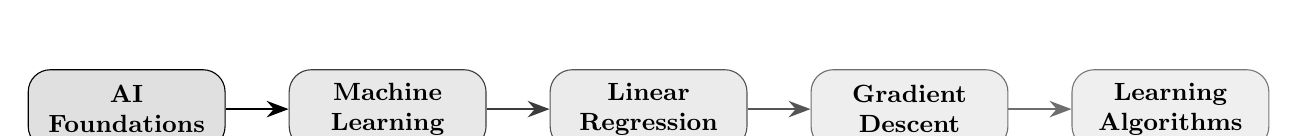
\begin{tikzpicture}[
  node distance=0.5cm,
  box/.style={rectangle, rounded corners=8pt, draw=#1, fill=#1!12,
    minimum width=2.5cm, minimum height=1cm, font=\small\bfseries, align=center},
  arrow/.style={-{Stealth[scale=1.2]}, thick, #1}
]
\node[box=primary] (ai) {AI\\Foundations};
\node[box=secondary, right=0.8cm of ai] (ml) {Machine\\Learning};
\node[box=accent, right=0.8cm of ml] (lr) {Linear\\Regression};
\node[box=highlight, right=0.8cm of lr] (gd) {Gradient\\Descent};
\node[box=purple, right=0.8cm of gd] (alg) {Learning\\Algorithms};

\draw[arrow=primary] (ai) -- (ml);
\draw[arrow=secondary] (ml) -- (lr);
\draw[arrow=accent] (lr) -- (gd);
\draw[arrow=highlight] (gd) -- (alg);
\end{tikzpicture}
}
\end{center}

\vfill
{\large\textcolor{primary}{\textbf{Department of Computer Science}}}\\[0.2cm]
{\normalsize\textcolor{darkgray}{Prepared for Academic Study}}
\end{titlepage}

%===============================================================================
% TABLE OF CONTENTS
%===============================================================================
\tableofcontents
\newpage

%===============================================================================
\chapter{Introduction to Artificial Intelligence}
%===============================================================================

\section{What is Artificial Intelligence?}

\begin{defbox}{Artificial Intelligence (AI)}
Artificial Intelligence is the branch of computer science concerned with building systems that can perform tasks that would normally require human intelligence. These tasks include reasoning, learning, planning, perception, language understanding, and problem solving.
\end{defbox}

AI can be broadly understood through two lenses:
\begin{itemize}[noitemsep]
  \item \textbf{Acting humanly:} Systems that behave as a human would (Turing test approach)
  \item \textbf{Acting rationally:} Systems that make optimal decisions given available information
  \item \textbf{Thinking humanly:} Cognitive modelling approach mimicking human thought
  \item \textbf{Thinking rationally:} Laws-of-thought approach using logic
\end{itemize}

\section{Contemporary Applications of AI}

AI is no longer a theoretical discipline --- it is embedded in everyday life:

\begin{center}
\resizebox{\textwidth}{!}{%
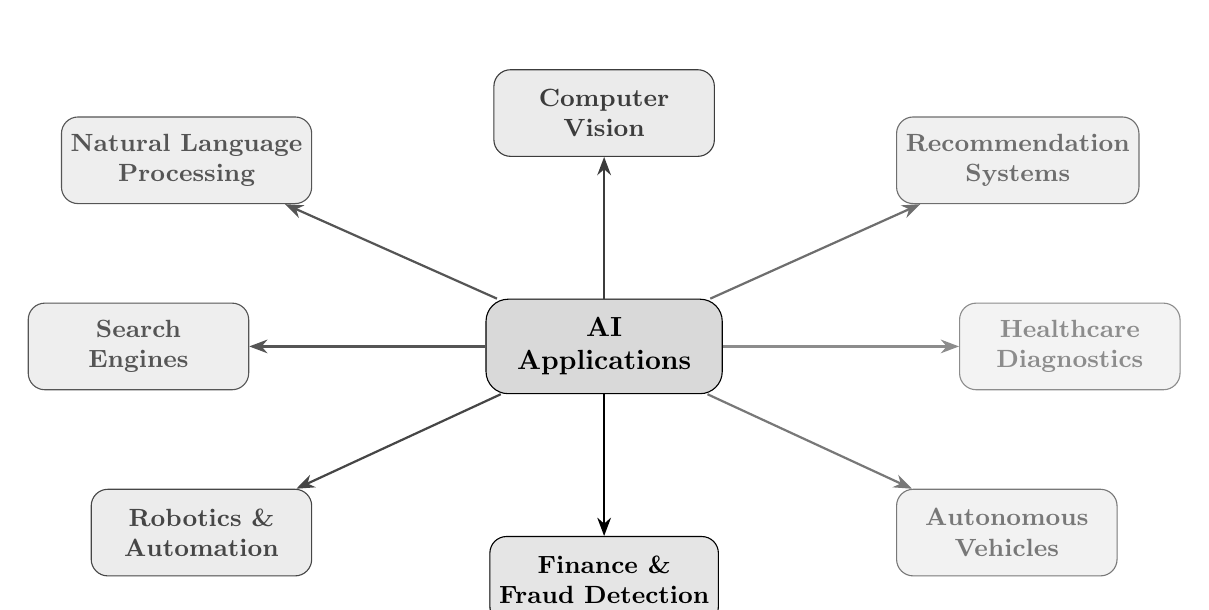
\begin{tikzpicture}[
  node distance=0.6cm,
  app/.style={rectangle, rounded corners=6pt, draw=#1, fill=#1!10,
    minimum width=2.8cm, minimum height=1.1cm, font=\small\bfseries\color{#1}, align=center},
  arrow/.style={-{Stealth}, thick, #1}
]
% Central node
\node[rectangle, rounded corners=8pt, draw=primary, fill=primary!15,
  minimum width=3cm, minimum height=1.2cm, font=\normalsize\bfseries\color{primary}, align=center] (ai) {AI\\Applications};

% Surrounding applications
\node[app=accent, above left=1.2cm and 2.2cm of ai] (nlp) {Natural Language\\Processing};
\node[app=secondary, above=1.8cm of ai] (cv) {Computer\\Vision};
\node[app=highlight, above right=1.2cm and 2.2cm of ai] (rec) {Recommendation\\Systems};
\node[app=danger, right=3cm of ai] (health) {Healthcare\\Diagnostics};
\node[app=purple, below right=1.2cm and 2.2cm of ai] (auto) {Autonomous\\Vehicles};
\node[app=primary, below=1.8cm of ai] (fin) {Finance \&\\Fraud Detection};
\node[app=darkgray, below left=1.2cm and 2.2cm of ai] (robot) {Robotics \&\\Automation};
\node[app=accent, left=3cm of ai] (search) {Search\\Engines};

\draw[arrow=accent] (ai) -- (nlp);
\draw[arrow=secondary] (ai) -- (cv);
\draw[arrow=highlight] (ai) -- (rec);
\draw[arrow=danger] (ai) -- (health);
\draw[arrow=purple] (ai) -- (auto);
\draw[arrow=primary] (ai) -- (fin);
\draw[arrow=darkgray] (ai) -- (robot);
\draw[arrow=accent] (ai) -- (search);
\end{tikzpicture}
}
\end{center}

\vspace{0.3cm}

\begin{center}
\begin{tabular}{lll}
\toprule
\textbf{Domain} & \textbf{AI Application} & \textbf{Example} \\
\midrule
Healthcare & Disease detection & Cancer screening via imaging \\
Finance & Fraud detection & Credit card anomaly detection \\
Transport & Autonomous driving & Tesla Autopilot, Waymo \\
Entertainment & Recommendation & Netflix, Spotify \\
Language & Translation \& chatbots & Google Translate, ChatGPT \\
Manufacturing & Quality control & Defect detection via vision \\
\bottomrule
\end{tabular}
\end{center}

\section{Strong AI vs.\ Weak AI}

\begin{tcolorbox}[colback=light, colframe=primary, boxrule=1.5pt, arc=6pt]
\begin{tabular}{p{0.45\textwidth}p{0.05\textwidth}p{0.45\textwidth}}
\textbf{\textcolor{primary}{Weak AI (Narrow AI)}} & & \textbf{\textcolor{danger}{Strong AI (General AI)}} \\[0.2cm]
Designed for a specific task & & Capable of any intellectual task a human can do \\
Operates within predefined domain & & Self-aware, conscious, general reasoning \\
Examples: Siri, chess engines, spam filters & & Hypothetical --- not yet achieved \\
Currently prevalent and practical & & Remains a long-term research goal \\
\end{tabular}
\end{tcolorbox}

\begin{keybox}
\textbf{Key Insight:} All AI systems today are \emph{Weak AI}. Strong AI (Artificial General Intelligence, AGI) remains a theoretical goal. The distinction matters for setting realistic expectations about what AI can and cannot do.
\end{keybox}

\section{History of AI}

\begin{center}
\resizebox{\textwidth}{!}{%
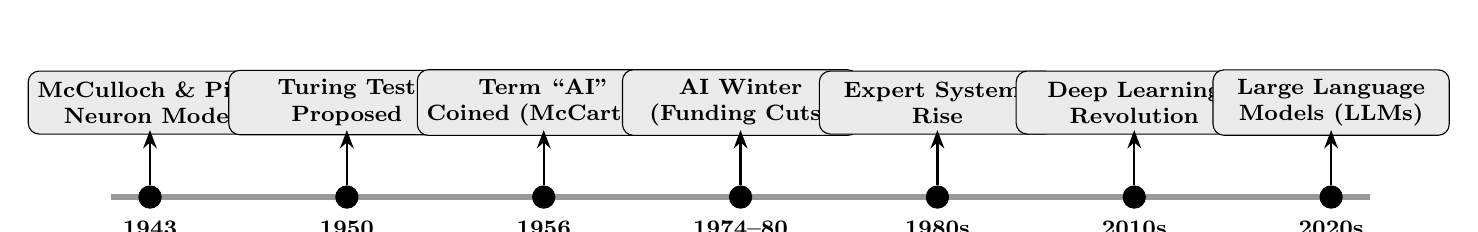
\begin{tikzpicture}[
  event/.style={rectangle, rounded corners=4pt, draw=primary, fill=primary!8,
    minimum width=3cm, minimum height=0.8cm, font=\footnotesize\bfseries, align=center},
  yr/.style={font=\footnotesize\bfseries\color{primary}},
  arrow/.style={-{Stealth}, thick, primary}
]
% Timeline line
\draw[line width=2pt, primary!40] (0,0) -- (16,0);

% Events
\node[event] at (0.5,1.2) (e1) {McCulloch \& Pitts\\Neuron Model};
\node[yr] at (0.5,-0.4) {1943};

\node[event] at (3,1.2) (e2) {Turing Test\\Proposed};
\node[yr] at (3,-0.4) {1950};

\node[event] at (5.5,1.2) (e3) {Term ``AI''\\Coined (McCarthy)};
\node[yr] at (5.5,-0.4) {1956};

\node[event] at (8,1.2) (e4) {AI Winter\\(Funding Cuts)};
\node[yr] at (8,-0.4) {1974--80};

\node[event] at (10.5,1.2) (e5) {Expert Systems\\Rise};
\node[yr] at (10.5,-0.4) {1980s};

\node[event] at (13,1.2) (e6) {Deep Learning\\Revolution};
\node[yr] at (13,-0.4) {2010s};

\node[event] at (15.5,1.2) (e7) {Large Language\\Models (LLMs)};
\node[yr] at (15.5,-0.4) {2020s};

% Dots on timeline
\foreach \x in {0.5,3,5.5,8,10.5,13,15.5}
  \filldraw[primary] (\x,0) circle (4pt);

% Arrows
\foreach \n/\x in {e1/0.5, e2/3, e3/5.5, e4/8, e5/10.5, e6/13, e7/15.5}
  \draw[arrow] (\x, 0.15) -- (\x, 0.85);

\end{tikzpicture}
}
\end{center}

\section{AI Controversies}

\begin{itemize}
  \item \textbf{Bias and Fairness:} AI models trained on biased data perpetuate discrimination (e.g., facial recognition performing poorly on darker skin tones).
  \item \textbf{Privacy:} Mass surveillance and data collection by AI systems raise civil liberties concerns.
  \item \textbf{Job Displacement:} Automation threatens certain categories of employment.
  \item \textbf{Autonomous Weapons:} Lethal autonomous weapons systems (LAWS) raise profound ethical questions.
  \item \textbf{Deepfakes:} AI-generated media can be used to spread disinformation.
  \item \textbf{Black-box Problem:} Many modern AI systems (deep neural networks) are not interpretable.
\end{itemize}

%===============================================================================
\chapter{Classical AI: Chatbots and the Turing Test}
%===============================================================================

\section{The Turing Test}

\begin{defbox}{Turing Test (1950)}
Proposed by Alan Turing in his paper \textit{"Computing Machinery and Intelligence"}, the Turing Test evaluates whether a machine can exhibit intelligent behaviour indistinguishable from that of a human. A human judge converses with both a human and a machine via text. If the judge cannot reliably distinguish which is which, the machine is said to have passed the test.
\end{defbox}

\begin{center}
\resizebox{0.7\textwidth}{!}{%
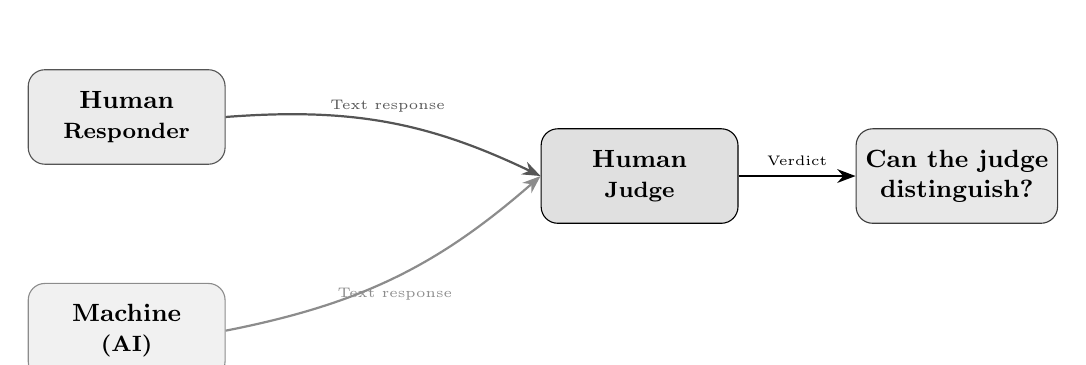
\begin{tikzpicture}[
  box/.style={rectangle, rounded corners=6pt, draw=#1, fill=#1!12,
    minimum width=2.5cm, minimum height=1.2cm, font=\small\bfseries, align=center},
  arrow/.style={-{Stealth}, thick}
]
\node[box=accent] (human) {Human\\\footnotesize Responder};
\node[box=danger, below=1.5cm of human] (machine) {Machine\\\footnotesize (AI)};
\node[box=primary, right=4cm of human, yshift=-0.75cm] (judge) {Human\\\footnotesize Judge};
\node[box=secondary, right=8cm of human, yshift=-0.75cm] (result) {Can the judge\\distinguish?};

\draw[-{Stealth}, thick, accent] (human.east) to[bend left=15] node[above, font=\tiny] {Text response} (judge.west);
\draw[-{Stealth}, thick, danger] (machine.east) to[bend right=15] node[below, font=\tiny] {Text response} (judge.west);
\draw[-{Stealth}, thick, primary] (judge.east) -- node[above, font=\tiny] {Verdict} (result.west);
\end{tikzpicture}
}
\end{center}

\subsection{Objections to the Turing Test}

\begin{enumerate}
  \item \textbf{Chinese Room Argument (Searle, 1980):} A system can appear to understand language by manipulating symbols according to rules without actually \emph{understanding} anything. Simulation $\neq$ intelligence.
  \item \textbf{It measures imitation, not intelligence:} Passing requires deception skills, not genuine cognition.
  \item \textbf{Human cognition as the wrong benchmark:} Intelligence need not resemble human intelligence.
  \item \textbf{No standard judge:} Results vary with different judges and contexts.
  \item \textbf{Narrow scope:} Only tests linguistic behaviour, ignoring vision, motor skills, and emotional intelligence.
\end{enumerate}

\section{Classical Chatbots}

\subsection{ELIZA (1966)}

\begin{defbox}{ELIZA}
Developed by Joseph Weizenbaum at MIT, ELIZA was one of the first natural language processing programs. Its most famous script, \textbf{DOCTOR}, simulated a Rogerian psychotherapist by applying simple pattern matching and scripted responses. It had no understanding of the conversation --- it simply reflected statements back as questions.
\end{defbox}

\begin{examplebox}{ELIZA Interaction}
\begin{tabular}{ll}
\textbf{User:} & ``I feel that nobody cares about me.'' \\
\textbf{ELIZA:} & ``Why do you feel that nobody cares about you?'' \\[0.2cm]
\textbf{User:} & ``My mother never listened to me.'' \\
\textbf{ELIZA:} & ``Tell me more about your family.'' \\
\end{tabular}

\vspace{0.2cm}
\textit{Key mechanism:} ELIZA looks for keywords like ``mother,'' ``feel,'' ``nobody'' and applies transformation templates to the user's input.
\end{examplebox}

\subsection{ALICE (Artificial Linguistic Internet Computer Entity)}

\begin{defbox}{ALICE}
Created by Richard Wallace in 1995, ALICE uses \textbf{AIML (Artificial Intelligence Markup Language)} --- an XML-based language for defining conversation rules. ALICE won the Loebner Prize (a Turing Test competition) three times (2000, 2001, 2004). It is a far more sophisticated pattern-matching system than ELIZA but still lacks genuine understanding.
\end{defbox}

\begin{examplebox}{ALICE/AIML Rule Structure}
\texttt{<category>}\\
\quad\texttt{<pattern>WHAT IS YOUR NAME</pattern>}\\
\quad\texttt{<template>My name is ALICE.</template>}\\
\texttt{</category>}
\vspace{0.2cm}

The pattern matches the user query; the template is the fixed response.
\end{examplebox}

\subsection{Kuki (formerly Mitsuku)}

\begin{defbox}{Kuki}
Kuki, originally named Mitsuku, was created by Steve Worswick using AIML. It is one of the most advanced retrieval-based chatbots, having won the Loebner Prize five times. It maintains a consistent persona, handles multi-turn conversations better than ELIZA or ALICE, and can perform simple reasoning tasks. It is freely available at \texttt{kuki.ai}.
\end{defbox}

\begin{center}
\begin{tabular}{llll}
\toprule
\textbf{Chatbot} & \textbf{Year} & \textbf{Mechanism} & \textbf{Notable Feature} \\
\midrule
ELIZA & 1966 & Pattern matching (scripts) & Rogerian therapist simulation \\
ALICE & 1995 & AIML rule-based & Loebner Prize winner (3x) \\
Kuki & 2005 & Advanced AIML & Loebner Prize winner (5x) \\
\bottomrule
\end{tabular}
\end{center}

%===============================================================================
\chapter{Symbolic AI and the Physical Symbol System Hypothesis}
%===============================================================================

\section{Symbolic AI}

\begin{defbox}{Symbolic AI}
Symbolic AI (also called Good Old-Fashioned AI, or \textbf{GOFAI}) is an approach to AI based on the explicit representation of knowledge as symbols and the manipulation of those symbols according to formal rules. It includes expert systems, logic-based reasoning, and rule-based systems.
\end{defbox}

Key characteristics:
\begin{itemize}[noitemsep]
  \item Knowledge is \textbf{explicitly encoded} as facts, rules, or ontologies
  \item Reasoning is performed through \textbf{logical inference}
  \item The system is \textbf{interpretable} --- you can trace every decision
  \item Struggles with \textbf{ambiguity, uncertainty, and learning from data}
\end{itemize}

\begin{examplebox}{Expert System: Medical Diagnosis}
\begin{tabular}{l}
\textbf{IF} patient has fever $>$ 38.5\textdegree C \\
\textbf{AND} patient has cough \\
\textbf{AND} patient has fatigue \\
\textbf{THEN} possible diagnosis = Influenza \\
\end{tabular}

Such rule-based systems (like MYCIN in the 1970s) could diagnose diseases at expert level but could not learn from new cases without manual rule updates.
\end{examplebox}

\section{Physical Symbol System Hypothesis (PSSH)}

\begin{defbox}{Physical Symbol System Hypothesis (Newell \& Simon, 1976)}
``\textit{A physical symbol system has the necessary and sufficient means for general intelligent action.}''\\[0.3cm]
This hypothesis asserts that:
\begin{enumerate}[noitemsep]
  \item Intelligence can be reduced to symbol manipulation.
  \item Any system capable of general intelligent action must be a physical symbol system.
  \item The brain is itself a physical symbol system.
\end{enumerate}
\end{defbox}

\subsection{What is a Physical Symbol System?}

A physical symbol system consists of:
\begin{itemize}[noitemsep]
  \item \textbf{Symbols:} Physical patterns (bits, words, tokens) that can be combined
  \item \textbf{Expressions:} Structures built from symbols
  \item \textbf{Processes:} Operations that create, modify, and destroy expressions
\end{itemize}

\begin{examplebox}{Physical Symbol System: Arithmetic}
Consider: $3 + 5 = 8$

\begin{tabular}{ll}
\textbf{Symbols:} & ``3'', ``+'', ``5'', ``='', ``8'' \\
\textbf{Expression:} & $3 + 5$ \\
\textbf{Process:} & Addition rule transforms $3 + 5 \rightarrow 8$ \\
\end{tabular}
\end{examplebox}

\subsection{Arguments For and Against PSSH}

\begin{center}
\begin{tabular}{p{0.45\textwidth}p{0.45\textwidth}}
\toprule
\textbf{\textcolor{accent}{For PSSH}} & \textbf{\textcolor{danger}{Against PSSH}} \\
\midrule
Successful expert systems in narrow domains & Fails to handle common-sense reasoning \\
Formal logic proved powerful for structured problems & Symbols have no inherent meaning (Searle) \\
Turing machines are symbol systems that are universal & Human cognition may not be symbolic at all \\
Language appears symbolic in structure & Frame problem: cannot handle dynamic real world \\
\bottomrule
\end{tabular}
\end{center}

%===============================================================================
\chapter{Introduction to Machine Learning}
%===============================================================================

\section{Datasets, Variables, and Features}

\begin{defbox}{Dataset}
A \textbf{dataset} is a structured collection of data points (observations or samples), where each data point is described by a set of \textbf{features} (also called variables or attributes) and often an associated \textbf{label} or \textbf{target value}.
\end{defbox}

\begin{examplebox}{House Price Dataset}
\begin{center}
\begin{tabular}{ccccl}
\toprule
\textbf{Size (m$^2$)} & \textbf{Bedrooms} & \textbf{Age (years)} & \textbf{Location} & \textbf{Price (\$)} \\
\midrule
85 & 3 & 10 & Urban & 250,000 \\
120 & 4 & 5 & Suburban & 320,000 \\
60 & 2 & 25 & Rural & 150,000 \\
200 & 5 & 2 & Urban & 600,000 \\
\bottomrule
\end{tabular}
\end{center}
\vspace{0.2cm}
\textbf{Features (inputs):} Size, Bedrooms, Age, Location \quad|\quad \textbf{Target (output):} Price
\end{examplebox}

\subsection{Types of Variables}

\begin{center}
\begin{tabular}{lll}
\toprule
\textbf{Type} & \textbf{Description} & \textbf{Example} \\
\midrule
Continuous & Any real number value & Height, Temperature, Price \\
Discrete & Integer or countable value & Number of bedrooms \\
Categorical (Nominal) & No natural ordering & Color (Red, Blue, Green) \\
Categorical (Ordinal) & Has natural ordering & Ratings (Low, Medium, High) \\
Binary & Only two values & Spam (Yes/No), Gender \\
\bottomrule
\end{tabular}
\end{center}

\subsection{Key Terminology}

\begin{itemize}[noitemsep]
  \item \textbf{Feature} ($x$): An input variable used to make predictions
  \item \textbf{Target / Label} ($y$): The output we want to predict
  \item \textbf{Sample / Observation} ($x^{(i)}, y^{(i)}$): A single data point
  \item \textbf{Training set:} Data used to fit the model
  \item \textbf{Test set:} Data used to evaluate model performance
  \item \textbf{Feature vector:} $\mathbf{x} = [x_1, x_2, \ldots, x_n]^T$

\end{itemize}

\section{Categories of Learning Algorithms}

\begin{center}
\resizebox{\textwidth}{!}{%
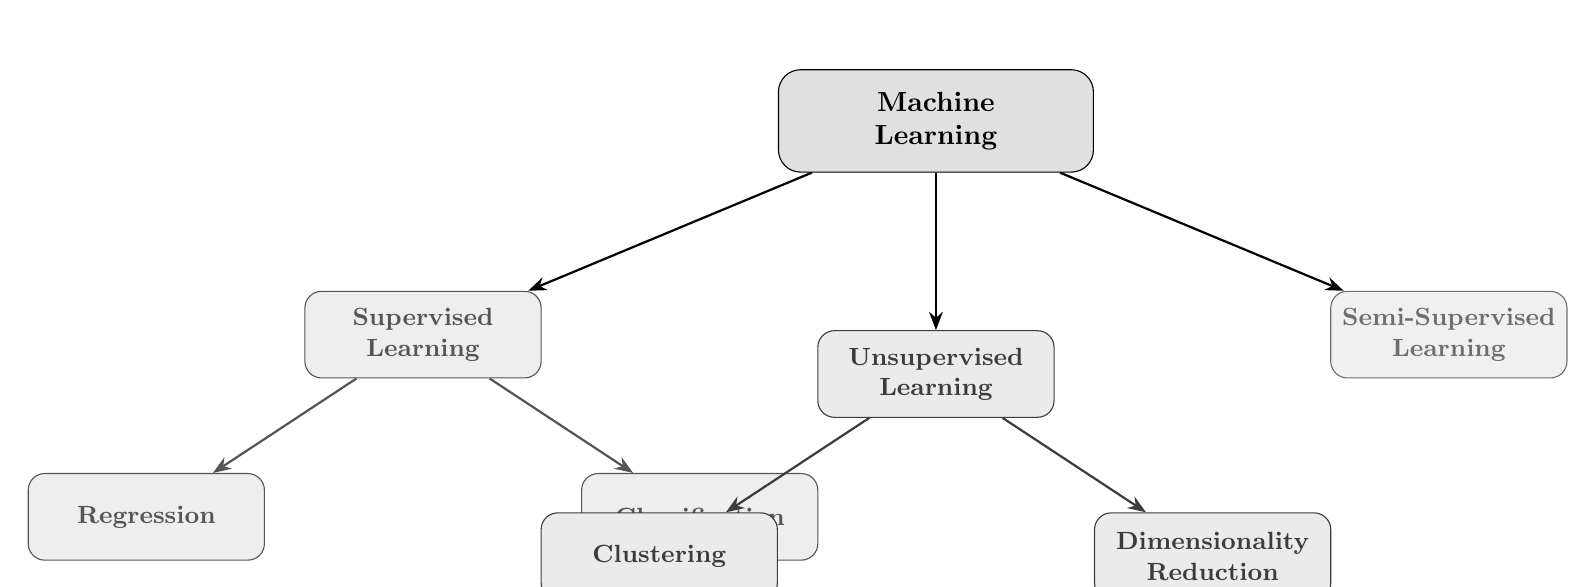
\begin{tikzpicture}[
  node distance=0.5cm,
  box/.style={rectangle, rounded corners=6pt, draw=#1, fill=#1!10,
    minimum width=3cm, minimum height=1.1cm, font=\small\bfseries\color{#1}, align=center},
  arrow/.style={-{Stealth}, thick, #1}
]
\node[rectangle, rounded corners=8pt, draw=primary, fill=primary!12,
  minimum width=4cm, minimum height=1.3cm, font=\normalsize\bfseries\color{primary}, align=center] (ml) {Machine\\Learning};

\node[box=accent, below left=1.5cm and 3cm of ml] (sup) {Supervised\\Learning};
\node[box=secondary, below=2cm of ml] (unsup) {Unsupervised\\Learning};
\node[box=highlight, below right=1.5cm and 3cm of ml] (semi) {Semi-Supervised\\Learning};

% Sub-nodes for supervised
\node[box=accent, below left=1.2cm and 0.5cm of sup] (reg) {Regression};
\node[box=accent, below right=1.2cm and 0.5cm of sup] (cls) {Classification};

% Sub-nodes for unsupervised
\node[box=secondary, below left=1.2cm and 0.5cm of unsup] (clu) {Clustering};
\node[box=secondary, below right=1.2cm and 0.5cm of unsup] (dr) {Dimensionality\\Reduction};

\draw[arrow=primary] (ml) -- (sup);
\draw[arrow=primary] (ml) -- (unsup);
\draw[arrow=primary] (ml) -- (semi);

\draw[arrow=accent] (sup) -- (reg);
\draw[arrow=accent] (sup) -- (cls);
\draw[arrow=secondary] (unsup) -- (clu);
\draw[arrow=secondary] (unsup) -- (dr);
\end{tikzpicture}
}
\end{center}

\section{Supervised Learning}

\begin{defbox}{Supervised Learning}
In supervised learning, the algorithm is trained on a \textbf{labelled dataset} --- each input $\mathbf{x}^{(i)}$ has a corresponding known output $y^{(i)}$. The goal is to learn a mapping $f: \mathbf{x} \rightarrow y$ that generalises to unseen data.
\end{defbox}

\subsection{Regression vs.\ Classification}

\begin{center}
\begin{tabular}{lll}
\toprule
 & \textbf{Regression} & \textbf{Classification} \\
\midrule
Output & Continuous value & Discrete class label \\
Example problem & Predict house price & Classify email as spam/not spam \\
Algorithms & Linear Regression, SVR, RF & Logistic Regression, SVM, KNN \\
Error metric & MSE, RMSE, MAE & Accuracy, F1-score, AUC \\
\bottomrule
\end{tabular}
\end{center}

\subsection{Common Supervised Learning Algorithms}

\begin{itemize}
  \item \textbf{Linear Regression:} Predicts a continuous output by fitting a linear relationship
  \item \textbf{Logistic Regression:} Predicts class probabilities using a sigmoid function
  \item \textbf{Decision Trees:} Partition the feature space using a tree structure
  \item \textbf{Random Forests:} Ensemble of decision trees to reduce overfitting
  \item \textbf{Support Vector Machines (SVM):} Finds the optimal hyperplane separating classes
  \item \textbf{K-Nearest Neighbours (KNN):} Classifies based on majority class of $k$ closest training points
  \item \textbf{Neural Networks:} Multi-layer non-linear transformations for complex patterns
\end{itemize}

\section{Unsupervised Learning}

\begin{defbox}{Unsupervised Learning}
In unsupervised learning, the algorithm is given \textbf{unlabelled data}. The goal is to discover hidden structure, patterns, or groupings within the data without explicit guidance.
\end{defbox}

\subsection{Common Unsupervised Algorithms}

\begin{itemize}
  \item \textbf{K-Means Clustering:} Partitions data into $k$ clusters by minimising within-cluster variance

    \begin{examplebox}{K-Means Example}
    Given customer purchase data (no labels), K-Means might discover natural customer segments: ``budget shoppers,'' ``premium buyers,'' and ``occasional buyers'' --- even though these labels were never provided.
    \end{examplebox}

  \item \textbf{DBSCAN:} Density-based clustering that can detect arbitrary-shaped clusters and outliers
  \item \textbf{Principal Component Analysis (PCA):} Reduces dimensionality by projecting onto axes of maximum variance
  \item \textbf{Autoencoders:} Neural networks that learn compressed representations of data
  \item \textbf{Gaussian Mixture Models (GMM):} Probabilistic model assuming data comes from multiple Gaussian distributions
\end{itemize}

\section{Semi-Supervised Learning}

\begin{defbox}{Semi-Supervised Learning}
Semi-supervised learning uses a \textbf{small amount of labelled data} combined with a \textbf{large amount of unlabelled data} for training. This is practical in real-world settings where labelling is expensive or time-consuming.
\end{defbox}

\begin{examplebox}{Semi-Supervised in Medical Imaging}
A hospital has 10,000 chest X-rays but only 500 have been reviewed by radiologists (labelled). Semi-supervised learning can use the pattern structure of all 10,000 images to improve a classifier trained only on the 500 labelled ones.
\end{examplebox}

\subsection{Approaches to Semi-Supervised Learning}

\begin{itemize}[noitemsep]
  \item \textbf{Self-training:} Train on labelled data, predict on unlabelled, add high-confidence predictions as pseudo-labels
  \item \textbf{Co-training:} Train multiple models on different feature subsets, each labelling data for the other
  \item \textbf{Graph-based:} Propagate labels through a graph where similar points are connected
  \item \textbf{Generative models:} Use VAEs or GANs to model the data distribution
\end{itemize}

\begin{center}
\begin{tabular}{llll}
\toprule
\textbf{Learning Type} & \textbf{Labels} & \textbf{Data} & \textbf{Use Case} \\
\midrule
Supervised & All labelled & Any amount & Abundant labels available \\
Unsupervised & None & Unlabelled & No labels exist \\
Semi-supervised & Few labelled & Mostly unlabelled & Labelling is expensive \\
\bottomrule
\end{tabular}
\end{center}

%===============================================================================
\chapter{Linear Regression}
%===============================================================================

\section{Introduction to Linear Regression}

\begin{defbox}{Linear Regression}
Linear regression is a \textbf{supervised learning algorithm} that models the relationship between one or more input features and a continuous output variable by fitting a linear (straight-line) equation to the data.
\end{defbox}

The model assumes the output $y$ is a linear function of the inputs:

\begin{formulabox}{Simple Linear Regression Model}
\[
\hat{y} = w_0 + w_1 x
\]
where:
\begin{itemize}[noitemsep]
  \item $\hat{y}$ = predicted output (dependent variable)
  \item $x$ = input feature (independent variable)
  \item $w_1$ = \textbf{weight} (slope) --- how much $y$ changes per unit change in $x$
  \item $w_0$ = \textbf{bias} (intercept) --- value of $\hat{y}$ when $x = 0$
\end{itemize}
\end{formulabox}

\begin{examplebox}{House Price Prediction (Simple Linear Regression)}
Predicting house price ($y$) from size in m$^2$ ($x$):

\[
\hat{y} = 1500 + 2500 \cdot x
\]

\begin{tabular}{cll}
$x = 80$ m$^2$: & $\hat{y} = 1500 + 2500 \times 80 = \$201{,}500$ \\
$x = 120$ m$^2$: & $\hat{y} = 1500 + 2500 \times 120 = \$301{,}500$ \\
\end{tabular}

Interpretation: Each additional m$^2$ adds \$2,500 to the predicted price.
\end{examplebox}

\begin{center}
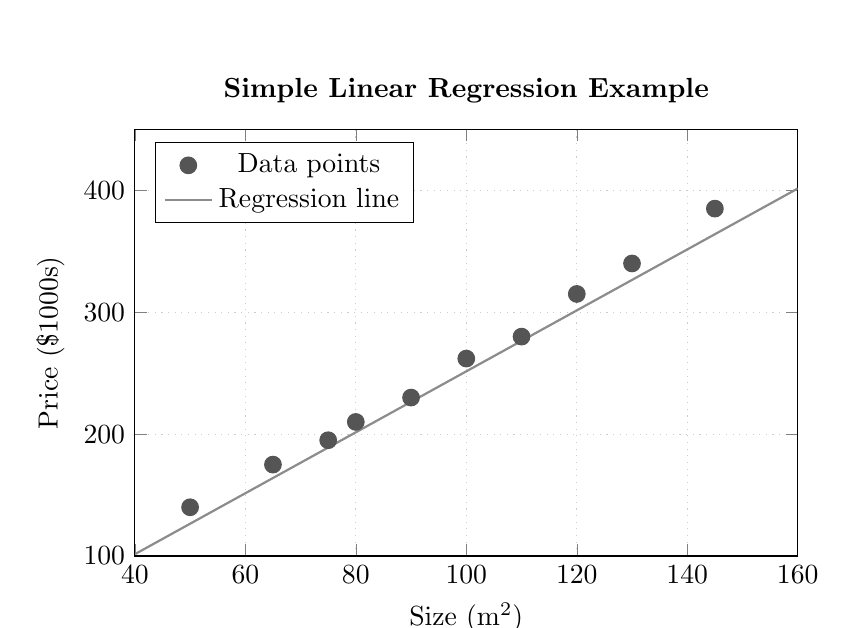
\begin{tikzpicture}
\begin{axis}[
  width=10cm, height=7cm,
  xlabel={Size (m$^2$)},
  ylabel={Price (\$1000s)},
  title={Simple Linear Regression Example},
  grid=major,
  grid style={dotted, gray!40},
  xmin=40, xmax=160,
  ymin=100, ymax=450,
  xtick={40,60,80,100,120,140,160},
  legend pos=north west,
  title style={color=primary, font=\bfseries},
  axis line style={primary},
]
% Data points
\addplot[only marks, mark=*, mark size=3pt, color=accent]
  coordinates {(50,140) (65,175) (75,195) (80,210) (90,230) (100,262) (110,280) (120,315) (130,340) (145,385)};

% Regression line
\addplot[thick, color=danger, domain=40:160]
  {1.5 + 2.5*x};

\legend{Data points, Regression line}
\end{axis}
\end{tikzpicture}
\end{center}

\section{Multiple Linear Regression}

\begin{defbox}{Multiple Linear Regression}
Multiple linear regression extends simple linear regression to \textbf{multiple input features}:

\[
\hat{y} = w_0 + w_1 x_1 + w_2 x_2 + \cdots + w_n x_n = w_0 + \sum_{j=1}^{n} w_j x_j
\]

In matrix form: $\hat{\mathbf{y}} = \mathbf{X}\mathbf{w}$ (including bias as $w_0$ with $x_0 = 1$).
\end{defbox}

\begin{examplebox}{Multiple Linear Regression: House Price}
\[
\hat{y} = 10{,}000 + 2500 \cdot x_{\text{size}} + 15{,}000 \cdot x_{\text{bedrooms}} - 500 \cdot x_{\text{age}}
\]
\begin{tabular}{ll}
$w_1 = 2500$: & Each m$^2$ adds \$2,500 \\
$w_2 = 15{,}000$: & Each bedroom adds \$15,000 \\
$w_3 = -500$: & Each year of age reduces price by \$500 \\
\end{tabular}

For a 100 m$^2$, 3-bedroom, 10-year-old house:
\[
\hat{y} = 10{,}000 + 2500(100) + 15{,}000(3) - 500(10) = \$300{,}000
\]
\end{examplebox}

\subsection{Weights, Bias, and Parameters}

\begin{center}
\begin{tabular}{lll}
\toprule
\textbf{Term} & \textbf{Symbol} & \textbf{Role} \\
\midrule
Weight & $w_j$ & Scales feature $x_j$; captures its importance \\
Bias & $w_0$ or $b$ & Offset term; shifts the prediction up/down \\
Parameters & $\mathbf{w} = [w_0, w_1, \ldots, w_n]^T$ & All learnable quantities in the model \\
\bottomrule
\end{tabular}
\end{center}

The goal of training is to \textbf{estimate the best values} of weights $\mathbf{w}$ from the data.

\section{Loss Function and Cost Function}

\begin{defbox}{Loss Function vs.\ Cost Function}
\begin{itemize}[noitemsep]
  \item \textbf{Loss Function} $L(\hat{y}^{(i)}, y^{(i)})$: Measures the error on a \textbf{single} training example
  \item \textbf{Cost Function} $J(\mathbf{w})$: Measures the \textbf{average} loss over the \textbf{entire} training set
\end{itemize}
\end{defbox}

\subsection{Mean Squared Error (MSE)}

The most common loss for regression is the \textbf{Squared Error Loss}:

\begin{formulabox}{Squared Error Loss (single example)}
\[
L(\hat{y}^{(i)}, y^{(i)}) = \left( \hat{y}^{(i)} - y^{(i)} \right)^2
\]
\end{formulabox}

\begin{formulabox}{Mean Squared Error (MSE) Cost Function}
\[
J(\mathbf{w}) = \frac{1}{m} \sum_{i=1}^{m} \left( \hat{y}^{(i)} - y^{(i)} \right)^2 = \frac{1}{m} \sum_{i=1}^{m} \left( w_0 + w_1 x^{(i)} - y^{(i)} \right)^2
\]
where $m$ is the number of training examples.
\end{formulabox}

\begin{examplebox}{Computing MSE}
\begin{center}
\begin{tabular}{ccccr}
\toprule
$i$ & $x^{(i)}$ & $y^{(i)}$ & $\hat{y}^{(i)} = 2 + 3x$ & $(\hat{y}^{(i)} - y^{(i)})^2$ \\
\midrule
1 & 1 & 5 & 5 & 0 \\
2 & 2 & 8 & 8 & 0 \\
3 & 3 & 10 & 11 & 1 \\
4 & 4 & 15 & 14 & 1 \\
\bottomrule
\end{tabular}
\end{center}

\[
J(w_0=2, w_1=3) = \frac{1}{4}(0 + 0 + 1 + 1) = 0.5
\]
\end{examplebox}

\section{Explained and Unexplained Variation}

\begin{defbox}{Decomposition of Total Variation}
For any observation $y^{(i)}$ with mean $\bar{y}$:
\[
\underbrace{(y^{(i)} - \bar{y})}_{\text{Total deviation}} = \underbrace{(\hat{y}^{(i)} - \bar{y})}_{\text{Explained}} + \underbrace{(y^{(i)} - \hat{y}^{(i)})}_{\text{Unexplained (residual)}}
\]
\end{defbox}

\subsection{Sum of Squares}

\begin{formulabox}{Sum of Squares Decomposition}
\[
\underbrace{\sum_{i=1}^m (y^{(i)} - \bar{y})^2}_{SST \text{ (Total)}} = \underbrace{\sum_{i=1}^m (\hat{y}^{(i)} - \bar{y})^2}_{SSR \text{ (Regression/Explained)}} + \underbrace{\sum_{i=1}^m (y^{(i)} - \hat{y}^{(i)})^2}_{SSE \text{ (Error/Unexplained)}}
\]
\[
SST = SSR + SSE
\]
\end{formulabox}

\begin{center}
\begin{tabular}{lll}
\toprule
\textbf{Quantity} & \textbf{Formula} & \textbf{Meaning} \\
\midrule
$SST$ (Total Sum of Squares) & $\sum (y^{(i)} - \bar{y})^2$ & Total variability in $y$ \\
$SSR$ (Regression Sum of Squares) & $\sum (\hat{y}^{(i)} - \bar{y})^2$ & Variation explained by model \\
$SSE$ (Error Sum of Squares) & $\sum (y^{(i)} - \hat{y}^{(i)})^2$ & Variation not explained \\
\bottomrule
\end{tabular}
\end{center}

\section{Coefficient of Determination ($R^2$)}

\begin{formulabox}{Coefficient of Determination}
\[
R^2 = \frac{SSR}{SST} = 1 - \frac{SSE}{SST}
\]
\begin{itemize}[noitemsep]
  \item $R^2 = 1$: Perfect fit --- model explains all variation in $y$
  \item $R^2 = 0$: Model explains nothing; as good as predicting $\bar{y}$
  \item $R^2 < 0$: Model is worse than simply predicting the mean
\end{itemize}
\end{formulabox}

\begin{examplebox}{$R^2$ Calculation}
\begin{tabular}{ll}
$SST = 1000$ & (total variability in house prices) \\
$SSE = 150$ & (unexplained by our model) \\
$SSR = 850$ & (explained by size, bedrooms, age) \\
\end{tabular}
\[
R^2 = 1 - \frac{150}{1000} = 0.85
\]
\textbf{Interpretation:} Our model explains 85\% of the variability in house prices.
\end{examplebox}

\section{Correlation Coefficient}

\begin{formulabox}{Pearson Correlation Coefficient}
\[
r = \frac{\sum_{i=1}^{m}(x^{(i)} - \bar{x})(y^{(i)} - \bar{y})}{\sqrt{\sum_{i=1}^m (x^{(i)}-\bar{x})^2 \cdot \sum_{i=1}^m (y^{(i)}-\bar{y})^2}}
\]
\begin{itemize}[noitemsep]
  \item $r \in [-1, 1]$
  \item $r = 1$: Perfect positive linear correlation
  \item $r = -1$: Perfect negative linear correlation
  \item $r = 0$: No linear correlation
  \item \textbf{For simple linear regression:} $r^2 = R^2$
\end{itemize}
\end{formulabox}

%===============================================================================
\chapter{Gradient Descent and Parameter Estimation}
%===============================================================================

\section{The Optimization Problem}

\begin{defbox}{Optimization Problem in ML}
Training a machine learning model is fundamentally an \textbf{optimization problem}:

\[
\mathbf{w}^* = \arg\min_{\mathbf{w}} J(\mathbf{w})
\]

Find the parameter values $\mathbf{w}^*$ that \textbf{minimize} the cost function $J(\mathbf{w})$.
\end{defbox}

\subsection{Types of Optimization Problems}

\begin{itemize}
  \item \textbf{Unconstrained:} Minimize $J(\mathbf{w})$ with no restrictions on $\mathbf{w}$ (most ML problems)
  \item \textbf{Constrained:} Minimize $J(\mathbf{w})$ subject to $g(\mathbf{w}) \leq 0$ or $h(\mathbf{w}) = 0$ (e.g., SVM)
  \item \textbf{Objective function:} The function being optimized (also called loss or cost in ML)
\end{itemize}

\section{Gradient Descent}

\begin{defbox}{Gradient Descent}
Gradient descent is an \textbf{iterative first-order optimization algorithm} used to minimize a differentiable function $J(\mathbf{w})$. Starting from an initial guess, it repeatedly moves in the direction of \textbf{steepest descent} (negative gradient) until convergence.
\end{defbox}

\subsection{Intuition}

Imagine standing on a hilly landscape (the cost function surface) in thick fog. You want to reach the lowest valley (minimum cost). Gradient descent says: at each step, feel the slope under your feet and take a step in the direction that goes \textbf{downhill most steeply}.

\begin{center}
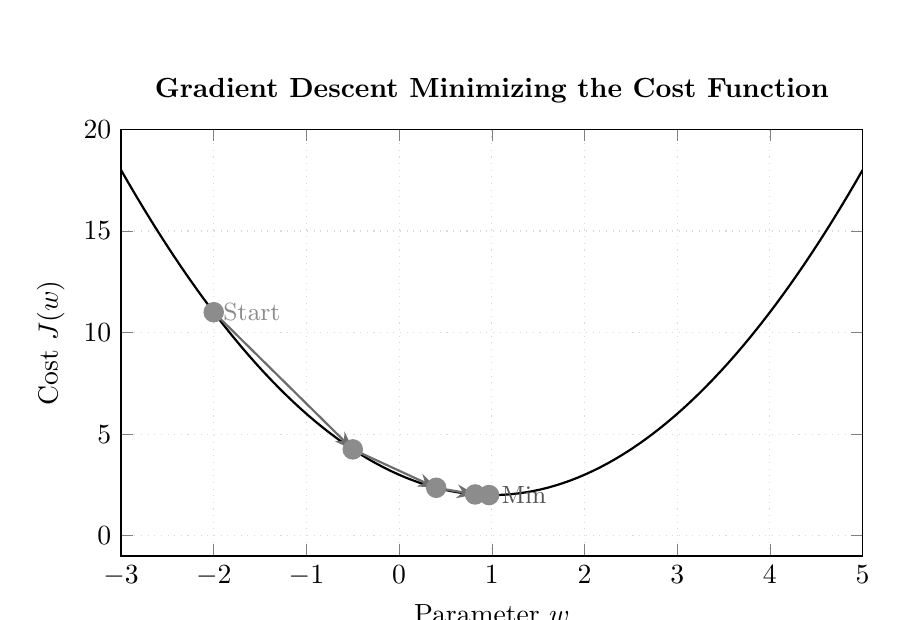
\begin{tikzpicture}
\begin{axis}[
  width=11cm, height=7cm,
  xlabel={Parameter $w$},
  ylabel={Cost $J(w)$},
  title={Gradient Descent Minimizing the Cost Function},
  title style={color=primary, font=\bfseries},
  grid=major,
  grid style={dotted, gray!30},
  xmin=-3, xmax=5,
  ymin=-1, ymax=20,
  domain=-3:5,
]
% Cost function: J(w) = (w-1)^2 + 2
\addplot[thick, color=primary, domain=-3:5, samples=100] {(x-1)^2 + 2};

% Gradient descent steps (manually placed)
\addplot[only marks, mark=*, mark size=3.5pt, color=danger]
  coordinates {(-2, 11) (-0.5, 4.25) (0.4, 2.36) (0.82, 2.032) (0.97, 2.0009)};

\addplot[-{Stealth}, thick, color=highlight]
  coordinates {(-2, 11) (-0.5, 4.25)};
\addplot[-{Stealth}, thick, color=highlight]
  coordinates {(-0.5, 4.25) (0.4, 2.36)};
\addplot[-{Stealth}, thick, color=highlight]
  coordinates {(0.4, 2.36) (0.82, 2.032)};
\addplot[-{Stealth}, thick, color=highlight]
  coordinates {(0.82, 2.032) (0.97, 2.0009)};

\node[font=\small, color=danger, anchor=west] at (axis cs:-2, 11) {Start};
\node[font=\small, color=accent, anchor=west] at (axis cs:1, 2) {Min};

\end{axis}
\end{tikzpicture}
\end{center}

\subsection{Gradient Descent Update Rule}

\begin{formulabox}{Gradient Descent Update Rule}
For each iteration $t$:
\[
w_j \leftarrow w_j - \alpha \cdot \frac{\partial J(\mathbf{w})}{\partial w_j}
\]
\begin{itemize}[noitemsep]
  \item $\alpha$ = \textbf{learning rate} (step size; hyperparameter)
  \item $\frac{\partial J}{\partial w_j}$ = partial derivative of cost w.r.t.\ weight $w_j$
  \item All weights are updated \textbf{simultaneously} in one pass
\end{itemize}
\end{formulabox}

\subsection{Gradients for Simple Linear Regression (MSE)}

Given $J(w_0, w_1) = \frac{1}{m}\sum_{i=1}^m (\hat{y}^{(i)} - y^{(i)})^2$ and $\hat{y}^{(i)} = w_0 + w_1 x^{(i)}$:

\begin{formulabox}{Partial Derivatives for Simple Linear Regression}
\[
\frac{\partial J}{\partial w_0} = \frac{2}{m} \sum_{i=1}^m \left( w_0 + w_1 x^{(i)} - y^{(i)} \right)
\]
\[
\frac{\partial J}{\partial w_1} = \frac{2}{m} \sum_{i=1}^m \left( w_0 + w_1 x^{(i)} - y^{(i)} \right) \cdot x^{(i)}
\]
\end{formulabox}

The update rules become:
\[
w_0 \leftarrow w_0 - \alpha \cdot \frac{2}{m} \sum_{i=1}^m (\hat{y}^{(i)} - y^{(i)})
\]
\[
w_1 \leftarrow w_1 - \alpha \cdot \frac{2}{m} \sum_{i=1}^m (\hat{y}^{(i)} - y^{(i)}) \cdot x^{(i)}
\]

\section{Gradient Ascent vs.\ Gradient Descent}

\begin{center}
\begin{tabular}{lll}
\toprule
 & \textbf{Gradient Descent} & \textbf{Gradient Ascent} \\
\midrule
Goal & \textbf{Minimize} $J(\mathbf{w})$ & \textbf{Maximize} $J(\mathbf{w})$ \\
Update rule & $w \leftarrow w - \alpha \nabla J$ & $w \leftarrow w + \alpha \nabla J$ \\
Direction & Moves \textbf{against} gradient & Moves \textbf{with} gradient \\
Use case & Loss minimization, regression & Reward maximization (RL), likelihood \\
\bottomrule
\end{tabular}
\end{center}

\begin{keybox}
\textbf{Key Insight:} Any maximization problem can be converted to minimization by negating the objective: $\max J(w) \equiv \min -J(w)$. In machine learning, we almost always minimize a cost/loss function, so gradient descent is the standard.
\end{keybox}

\section{Learning Rate: Effect on Convergence}

\begin{center}
\begin{tabular}{lll}
\toprule
\textbf{Learning Rate $\alpha$} & \textbf{Behaviour} & \textbf{Problem} \\
\midrule
Too large & Overshoots minimum & May diverge (cost increases) \\
Too small & Takes tiny steps & Very slow convergence \\
Just right & Steady convergence & Reaches minimum efficiently \\
\bottomrule
\end{tabular}
\end{center}

\section{Worked Example: Gradient Descent Iterations}

\begin{examplebox}{Step-by-Step Gradient Descent for Simple Linear Regression}
\textbf{Training data (4 points):}\\
$(1, 2),\ (2, 4),\ (3, 6),\ (4, 8)$ \quad (True relationship: $y = 2x$)

\textbf{Initial parameters:} $w_0 = 0,\ w_1 = 0$ \quad \textbf{Learning rate:} $\alpha = 0.01$

\vspace{0.3cm}
\textbf{Iteration 1:}

Predictions: $\hat{y}^{(i)} = 0 + 0 \cdot x = 0$ for all $i$

Errors: $(0-2), (0-4), (0-6), (0-8)$

\[
\frac{\partial J}{\partial w_0} = \frac{2}{4}\left[(-2)+(-4)+(-6)+(-8)\right] = \frac{2}{4}(-20) = -10
\]
\[
\frac{\partial J}{\partial w_1} = \frac{2}{4}\left[(-2)(1)+(-4)(2)+(-6)(3)+(-8)(4)\right] = \frac{2}{4}(-60) = -30
\]

Updates:
\[
w_0 \leftarrow 0 - 0.01 \times (-10) = 0.1
\]
\[
w_1 \leftarrow 0 - 0.01 \times (-30) = 0.3
\]

\vspace{0.3cm}

\begin{center}
\begin{tabular}{cccccc}
\toprule
\textbf{Iteration} & $w_0$ & $w_1$ & $J(w_0, w_1)$ & $\partial J/\partial w_0$ & $\partial J/\partial w_1$ \\
\midrule
0 (init) & 0.000 & 0.000 & 30.000 & $-10.0$ & $-30.0$ \\
1 & 0.100 & 0.300 & 20.155 & $-8.40$ & $-25.4$ \\
2 & 0.184 & 0.554 & 13.572 & $-7.07$ & $-21.4$ \\
3 & 0.255 & 0.768 & 9.148 & $-5.94$ & $-18.0$ \\
10 & 0.531 & 1.527 & 1.712 & $-2.50$ & $-7.6$ \\
50 & 0.982 & 1.967 & 0.003 & $-0.06$ & $-0.2$ \\
100 & 0.999 & 1.999 & $\approx 0$ & $\approx 0$ & $\approx 0$ \\
\bottomrule
\end{tabular}
\end{center}

\vspace{0.3cm}
After convergence: $w_0 \approx 0,\ w_1 \approx 2$ --- matching the true relationship $y = 2x$!
\end{examplebox}

\begin{center}
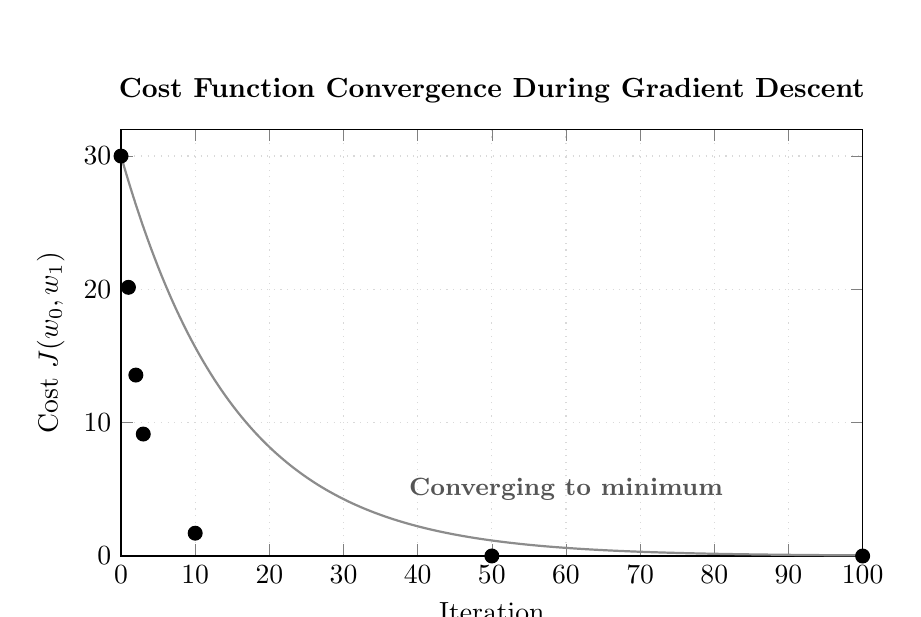
\begin{tikzpicture}
\begin{axis}[
  width=11cm, height=7cm,
  xlabel={Iteration},
  ylabel={Cost $J(w_0, w_1)$},
  title={Cost Function Convergence During Gradient Descent},
  title style={color=primary, font=\bfseries},
  grid=major,
  grid style={dotted, gray!30},
  xmin=0, xmax=100,
  ymin=0, ymax=32,
  domain=0:100,
]
\addplot[thick, color=danger, domain=0:100, samples=200]
  {30 * exp(-0.065*x) + 0.003};
\addplot[only marks, mark=*, mark size=2.5pt, color=primary]
  coordinates {(0,30) (1, 20.155) (2, 13.572) (3, 9.148) (10, 1.712) (50, 0.003) (100, 0)};

\node[font=\small\bfseries, color=accent] at (axis cs:60, 5) {Converging to minimum};
\end{axis}
\end{tikzpicture}
\end{center}

\section{Variants of Gradient Descent}

\begin{center}
\begin{tabular}{llll}
\toprule
\textbf{Variant} & \textbf{Batch Size} & \textbf{Update frequency} & \textbf{Noise} \\
\midrule
Batch GD & All $m$ samples & Once per epoch & None (smooth) \\
Stochastic GD (SGD) & 1 sample & $m$ times per epoch & High \\
Mini-Batch GD & $k$ samples ($1 < k < m$) & $m/k$ times per epoch & Moderate \\
\bottomrule
\end{tabular}
\end{center}

\begin{notebox}
Mini-batch gradient descent is the \textbf{standard in practice}: batch sizes of 32, 64, or 128 balance computational efficiency and convergence stability. Libraries like PyTorch and TensorFlow use mini-batch GD by default.
\end{notebox}

\section{Parameter Estimation: Analytical vs.\ Iterative}

For linear regression there exist two approaches to finding $\mathbf{w}^*$:

\subsection{Normal Equation (Analytical)}

\begin{formulabox}{Normal Equation}
\[
\mathbf{w}^* = (\mathbf{X}^T \mathbf{X})^{-1} \mathbf{X}^T \mathbf{y}
\]
\begin{itemize}[noitemsep]
  \item Directly computes the exact solution in one step
  \item Requires computing a matrix inverse: $O(n^3)$ complexity
  \item Impractical when $n$ (number of features) is very large
\end{itemize}
\end{formulabox}

\subsection{Gradient Descent (Iterative)}

\begin{formulabox}{Gradient Descent Parameter Estimation}
\[
\mathbf{w} \leftarrow \mathbf{w} - \alpha \nabla_{\mathbf{w}} J(\mathbf{w})
\]
\begin{itemize}[noitemsep]
  \item Iteratively approaches the solution
  \item Scales to large datasets and many features
  \item Requires tuning the learning rate $\alpha$
  \item Generalises to non-linear models (neural networks)
\end{itemize}
\end{formulabox}

\begin{center}
\begin{tabular}{lll}
\toprule
 & \textbf{Normal Equation} & \textbf{Gradient Descent} \\
\midrule
Speed & Fast for small $n$ & Scales to large $n$ \\
Hyperparameters & None & Needs $\alpha$, iterations \\
Invertibility & Fails if $\mathbf{X}^T\mathbf{X}$ singular & Always applicable \\
Generalisation & Linear models only & Any differentiable model \\
\bottomrule
\end{tabular}
\end{center}

%===============================================================================
\chapter{Summary and Key Formulas}
%===============================================================================

\section{Quick Reference: Key Formulas}

\begin{tcolorbox}[colback=light, colframe=primary, boxrule=2pt, arc=8pt, title=\textbf{Essential Formulas for Exam Review}, fonttitle=\bfseries\color{white}]

\textbf{Simple Linear Regression:}
\[ \hat{y} = w_0 + w_1 x \]

\textbf{Multiple Linear Regression:}
\[ \hat{y} = w_0 + w_1 x_1 + w_2 x_2 + \cdots + w_n x_n \]

\textbf{MSE Cost Function:}
\[ J(\mathbf{w}) = \frac{1}{m}\sum_{i=1}^{m}(\hat{y}^{(i)} - y^{(i)})^2 \]

\textbf{Gradient Descent Update:}
\[ w_j \leftarrow w_j - \alpha \cdot \frac{\partial J}{\partial w_j} \]

\textbf{Coefficient of Determination:}
\[ R^2 = 1 - \frac{SSE}{SST}, \quad SST = SSR + SSE \]

\textbf{Pearson Correlation:}
\[ r = \frac{\sum(x^{(i)}-\bar{x})(y^{(i)}-\bar{y})}{\sqrt{\sum(x^{(i)}-\bar{x})^2 \cdot \sum(y^{(i)}-\bar{y})^2}} \]

\textbf{Normal Equation:}
\[ \mathbf{w}^* = (\mathbf{X}^T\mathbf{X})^{-1}\mathbf{X}^T\mathbf{y} \]
\end{tcolorbox}

\section{Learning Algorithm Comparison}

\begin{center}
\begin{tabular}{llll}
\toprule
\textbf{Algorithm} & \textbf{Type} & \textbf{Output} & \textbf{Key Assumption} \\
\midrule
Linear Regression & Supervised & Continuous & Linear relationship \\
Logistic Regression & Supervised & Class label & Linear decision boundary \\
K-Nearest Neighbours & Supervised & Any & Proximity = similarity \\
Decision Tree & Supervised & Any & Greedy splits minimise impurity \\
K-Means & Unsupervised & Cluster ID & Spherical, equal clusters \\
PCA & Unsupervised & Components & Variance = information \\
Semi-supervised SVM & Semi-supervised & Class label & Unlabelled near boundary \\
\bottomrule
\end{tabular}
\end{center}

\vfill
\begin{tcolorbox}[colback=accent!10, colframe=accent, boxrule=1.5pt, arc=6pt]
\centering
\textbf{\large End of Study Notes}\\[0.2cm]
\normalsize These notes cover: Introduction to AI $\cdot$ Chatbots \& Turing Test $\cdot$ Symbolic AI $\cdot$ Linear Regression $\cdot$ Gradient Descent $\cdot$ Learning Algorithms
\end{tcolorbox}

\end{document}
